%% ++++++++++++++++++++++++++++++++++++++++++++++++++++++++++++
%% Kapitel 1: Einleitung
%% ++++++++++++++++++++++++++++++++++++++++++++++++++++++++++++


\chapter{Introduction}
In Global Navigation Satellite Systems (GNSS), including GPS, GNSS and GLONASS, the first step for the receiver is scanning all satellites insight. This process is called aquisition. Every satellite continuously transmit a signal contain the special Pseudo Random Code (PRN) belonging to satellite. By decoding this signal the receiver knows from which satellite the signal comes from. All possible PRN codes are stored in the receiver. One of the characteristic of the PRN is that they are completely orthogonal. Consequently, the correlation between the code and the received signal has if and only if a peak if it is exactly the same code. Because the code received within the signal can be time-shifted, this delay $\tau$ has to be searched to verify the satellite ID. 

There are two possible search strategies to get $ \tau $. The first method is a sequential search, where correlations for each $\tau$ are calculated and looked for a peak. If it is the wrong code only noise occur. For this I created a for-loop with an amount of different $\tau$ in steps of $ 1 / f_{s} =  977.52 \mu s$ corresponding to one chip. For each shifted code the correlation will be calculated with $ C = \mid(y^{T}\cdot c(\tau )\mid $ with $y^{T}$ being the transposed received signal and $c(\tau )$ the code signal shifted by $\tau$. Afterwards, the maximum correlation will be calculated, which corresponds to the searched $\tau$.

\begin{figure}[!ht]
\centering
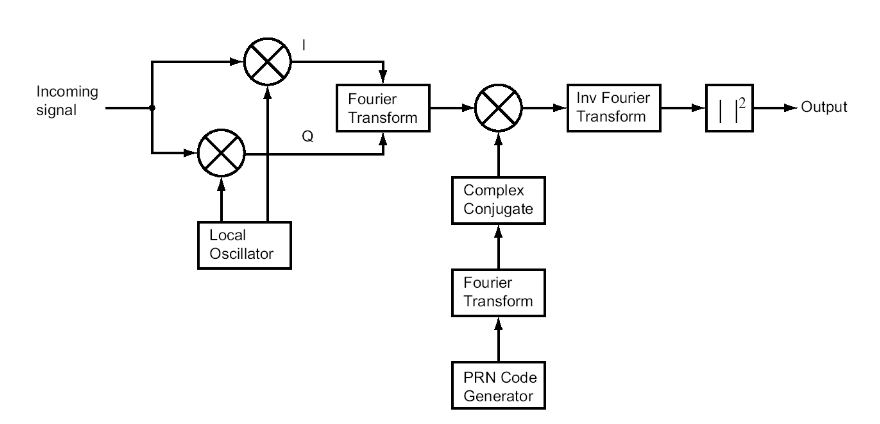
\includegraphics[scale=0.5]{bilder/method.png} 
\caption{Parallel Code Phase Search}
\label{bild:method}
\end{figure}

Another more time-efficient method is a parallel code phase search corresponding to \ref{bild:method}. This method uses the fast fourier transformation to search only for one loop. A correlation can be expressed like this formulation:

\[ C\left[ n = \triangle \tau \right] = y \left[ n \right] \bigotimes c \left[ \tau \right]  =  \sum \limits_{m=0}^{N-1}y\left[ m \right] \bigotimes c \left[n + m \right] \] 

After fourier transformation both signals can be multiplied:

\[C \left[ k \right]  =  Y\left[ k \right]  \cdot C^{ \ast } \left[ k \right]   \] 

and back transformed it corresponds to the correlation again.

\[C \left[ n \right]^{2}  =  F_{FFT}^{-1} \left\lbrace Y\left[ k \right]  \cdot C^{ \ast } \left[ k \right] \right\rbrace  ^{2}  \] 

By implementing this only the code with $ \tau $ = 0 has to be generated and transformed into the fourier domain as well as the received signal. Afterwards, the received signal with the conjugated complex code signal will be multiplied and back transformed.  Due to the calculation in frequency domain all different time-shifted correlations are calculated. The property of fourier transformation is exactly this time-shifting. After back-transformation you can see a plot of $ C\left[ m \right]  $ like \ref{bild:corr}. At the point of the peak is the searched $ \tau $. It is 400 $ T_{c} $ long. 

By comparing both methods the sequential search takes about 8 s while the parallel search only takes 50 ms. Therefore, the second method is much faster and thus more suitable. The restriction for the time, there, is only the algorithm of the fast fourier transform, which could be for example a Decimation-in-Frequency or Decimation-in-Time algorithm.

\begin{figure}[!ht]
\centering
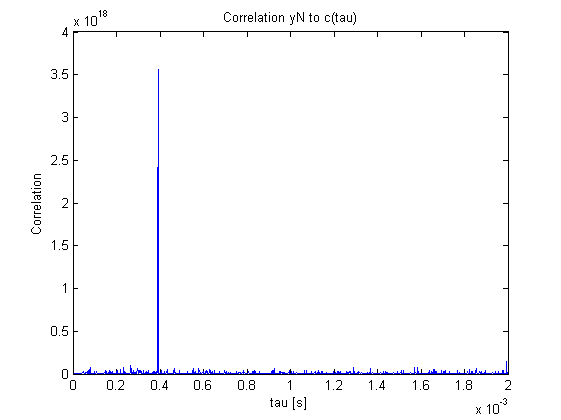
\includegraphics[scale=0.5]{bilder/results.png} 
\caption{Correlation over different $ \tau $}
\label{bild:corr}
\end{figure}